\setcounter{subsection}{0}
The first performance results we'll talk about is comparing our lock-free implementation of BQ compared to the performance of a standard implementation of a lock-free queue. The goal here was to measure overall run-time on 5000 operations of random enqueue and dequeue operations while also varying the batch size amount and amount of threads. In \textit{Figure 1} we see the smallest batch size of 4 perform about expected. With smaller batch sizes, BQ is not fully utilizing the performance increase of batching operations. With batch sizes this small, the standard lock-free queue slightly out performs BQ. 

\begin{figure}[htp]

\centering
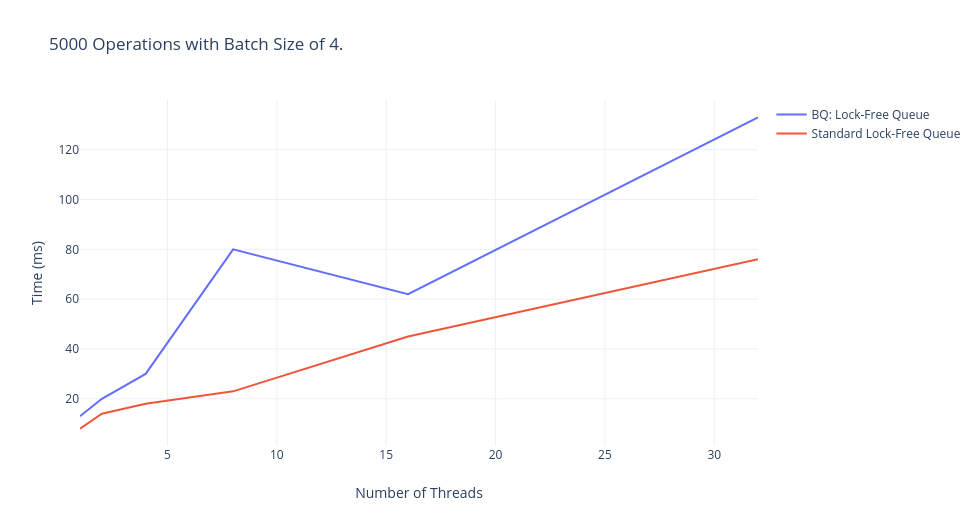
\includegraphics[height=6cm, width=13cm]{images/imgB64.png}\hfill
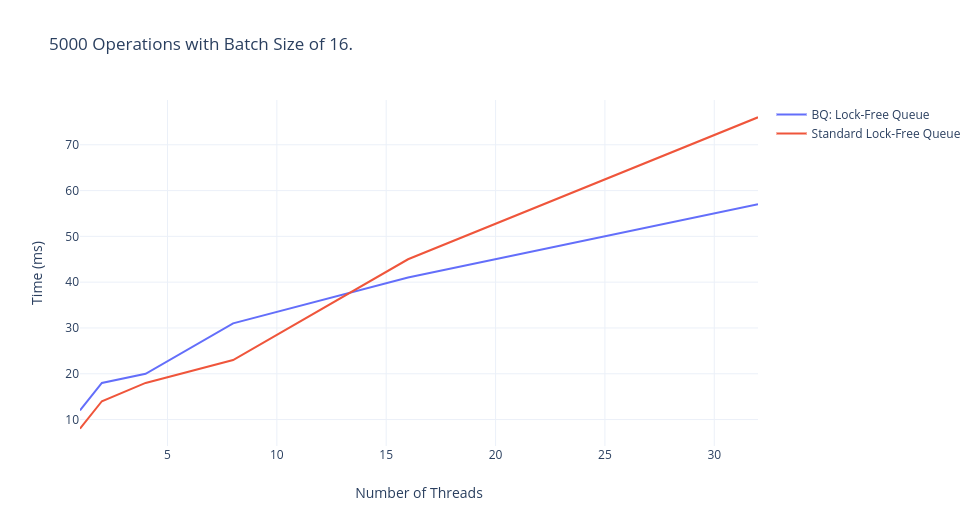
\includegraphics[height=6cm, width=13cm]{images/imgB16.png}\hfill
\newpage
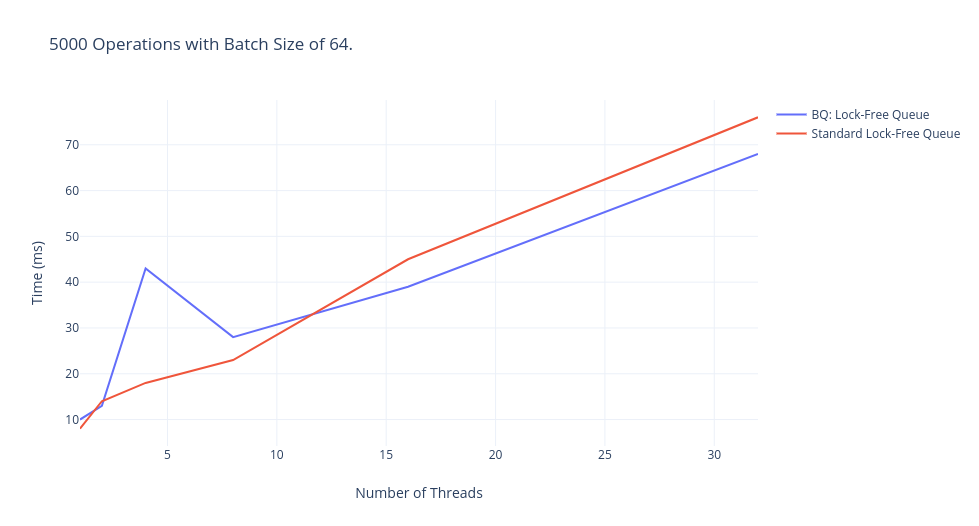
\includegraphics[height=6cm, width=13cm]{images/imgB4.png}\hfill

\caption{BQ vs Lock-Free Queue}
\label{fig:figure3}
\end{figure}
We start to see improvement over the standard lock-free implementation with a
batch size of 16. This result was expected because as the batch sizes increase so should the performance of BQ. The last graph is with a batch size of 64, and is where we see the biggest performance increase. Increasing the load from this point forward would just increase the performance of BQ compared to the lock-free queue. 